% Dummy comment so that files shows up in Reviewable.

\textit{Inverse dynamics} refers to the computation of the impulses given known
velocities of the system. It is shown in \cite{bib:todorov2014} that contact
impulses are solution to the convex program stated in Eq.
(\ref{eq:y_projection}). This problem can be solved analytically using simple
geometry. By noticing that the change of variables
$\tilde\bgamma=\vf{R}^{1/2}\bgamma$ (and respectively
$\tilde{\vf{y}}=\vf{R}^{1/2}\vf{y}$) leads to a projection with Euclidian norm
on a cone $\mathcal{F}_{\tilde\mu}$ with friction coefficient
$\tilde\mu=\mu\,(R_t/R_n)^{1/2}$
\begin{eqnarray}
	P_\mathcal{F_{\tilde\mu}}(\tilde{\vf{y}})&=&\argmin_{\tilde\bgamma\in\mathcal{F_{\tilde\mu}}}
		\quad \frac{1}{2}\Vert\tilde\bgamma-\tilde{\vf{y}}\Vert_2^2\nonumber\\
	P_\mathcal{F}(\vf{y}) &=&
	\vf{R}^{-1/2}P_\mathcal{F_{\tilde\mu}}(\tilde{\vf{y}})
	\label{eq:local_optimization_problem_tilde}
\end{eqnarray}

The optimization problem in the Euclidean norm given by Eq.
(\ref{eq:local_optimization_problem_tilde}) can be solved by inspection. If
$\tilde{\vf{y}}\in\mathcal{F}_{\tilde\mu}$, then we simply have $\tilde{\bgamma}
= \tilde{\vf{y}}$, we call this \textit{Region I}. If however $\tilde{\vf{y}}$
is inside the polar cone $\mathcal{F}_{\tilde\mu}^\circ$, the closest point to
$\tilde{\vf{y}}_i$ within the (tilde) friction cone is zero, i.e.
$\tilde{\bgamma} =\vf{0}$. We call this \textit{Region III}. Finally, if
$\tilde{\vf{y}}$ is in the region outside both $\mathcal{F}_{\tilde\mu}$ and its
polar $\mathcal{F}_{\tilde\mu}^\circ$, then the closest point is it's Euclidian
projection on the boundary of $\mathcal{F}_{\tilde\mu}$. We call this
\textit{Region II}. Figure \ref{fig:cone_regions} shows a schematic of
$\mathcal{F}_{\tilde\mu}$, $\mathcal{F}_{\tilde\mu}^\circ$ and labels the three
different regions. From Fig. \ref{fig:cone_regions}, for a cone forming an angle
$\theta$ with the z axis, we have $\tan(\theta)=\tilde\mu$ and
$\cos(\theta)=1/(1+\tilde\mu^2)$. Then the projection of a point
$\tilde{\vf{y}}$ in Region II can be written as
\begin{eqnarray}
	\tilde{\bgamma}_t &=& \tilde{\mu}\tilde{\gamma}_n\hat{\vf{t}}\nonumber\\
	\tilde{\gamma}_n &=& \frac{1}{1+\tilde{\mu}^2}\left(\tilde{y}_n +
	\tilde{\mu}\tilde{y}_r\right)\nonumber		
\end{eqnarray}
where the tangent vector is defined as
$\hat{\vf{t}}=\vf{y}_t/\Vert\vf{y}_t\Vert=-\vf{v}_t/\Vert\vf{v}_t\Vert$. 
\begin{figure}[!h]
    \centering
    %\vspace{6pt}
    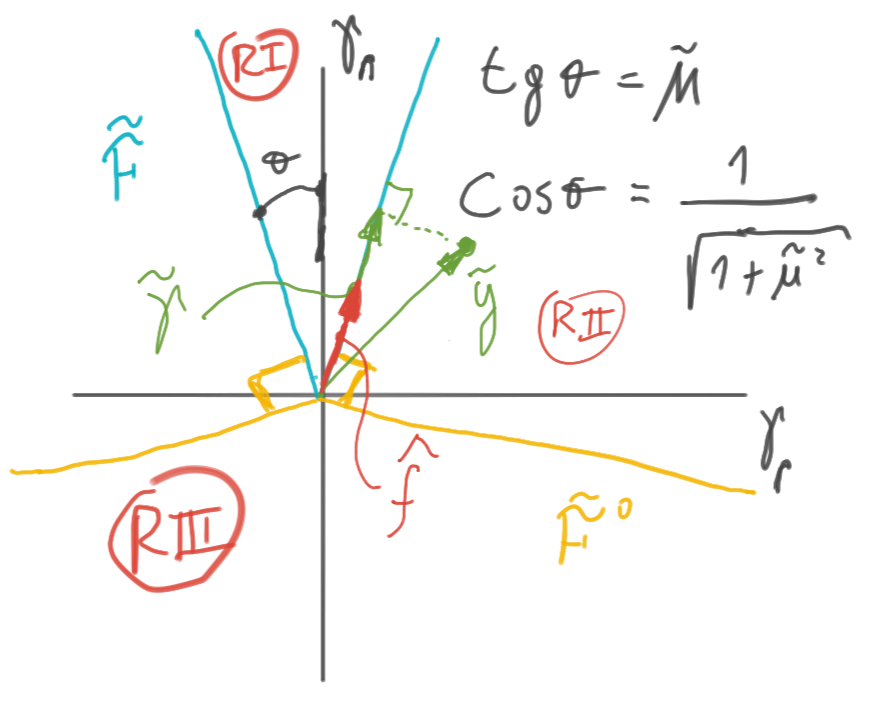
\includegraphics[width=0.45\columnwidth]{figures/cone_regions.png}
    \caption{Geometry of $\mathcal{F}_{\tilde\mu}$ and regions in the
    $\tilde{\vf{y}}$ space.}
    \label{fig:cone_regions}
\end{figure}

Finally, we obtain Eq. (\ref{eq:y_projection}) by applying the transformation
$\bgamma=\mf{R}^{-1/2}\tilde\bgamma$ to recover the impulses projected onto the
friction cone ${\mathcal{F}}_{\mu}$ using the norm in $\vf{R}$.

Though the tangent vector $\hat{\vf{t}}$ is not defined for $\vf{y}=\vf{0}$, the
projection still is, $P_\mathcal{F}(\vf{0})=\vf{0}$. In practice however, we
introduce a smooth \emph{soft-norm} defined as
$\|\vf{x}\|_s=\sqrt{\|\vf{x}\|^2+\varepsilon_s^2}$ and we define the tangent
vector as $\hat{\vf{t}}=\vf{y}_t/\Vert\vf{y}_t\Vert_s$. This newly defined tangent vector is smooth and has the desired property that it leads to the right
projection result in the limit to $\vf{y}\rightarrow 0$. In addition, not only
the projection is well defined, but also its gradients in Appendix
\ref{app:gradients_derivation}. In practice we use $\varepsilon_s=10^{-8}$.

